\documentclass[12pt, titlepage]{article}

\usepackage{amsmath, mathtools}

\usepackage[round]{natbib}
\usepackage{amsfonts}
\usepackage{amssymb}
\usepackage{graphicx}
\usepackage{colortbl}
\usepackage{xr}
\usepackage{hyperref}
\usepackage{longtable}
\usepackage{xfrac}
\usepackage{tabularx}
\usepackage{float}
\usepackage{siunitx}
\usepackage{booktabs}
\usepackage{multirow}
\usepackage[section]{placeins}
\usepackage{caption}
\usepackage{fullpage}

\hypersetup{
bookmarks=true,     % show bookmarks bar?
colorlinks=true,       % false: boxed links; true: colored links
linkcolor=red,          % color of internal links (change box color with linkbordercolor)
citecolor=blue,      % color of links to bibliography
filecolor=magenta,  % color of file links
urlcolor=cyan          % color of external links
}

\usepackage{array}

%% Comments

\usepackage{color}

\newif\ifcomments\commentstrue %displays comments
%\newif\ifcomments\commentsfalse %so that comments do not display

\ifcomments
\newcommand{\authornote}[3]{\textcolor{#1}{[#3 ---#2]}}
\newcommand{\todo}[1]{\textcolor{red}{[TODO: #1]}}
\else
\newcommand{\authornote}[3]{}
\newcommand{\todo}[1]{}
\fi

\newcommand{\wss}[1]{\authornote{blue}{SS}{#1}} 
\newcommand{\plt}[1]{\authornote{magenta}{TPLT}{#1}} %For explanation of the template
\newcommand{\an}[1]{\authornote{cyan}{Author}{#1}}

%% Common Parts

\newcommand{\progname}{Housemates} % PUT YOUR PROGRAM NAME HERE
\newcommand{\authname}{Team \#9, Housemates
\\ Justin Dang - dangj15 
\\ Harris Hamid - hamidh1
\\ Fady Morcos - morcof2 
\\ Rizwan Ahsan - ahsanm7
\\ Sheikh Afsar - afsars} % AUTHOR NAMES                  

\usepackage{hyperref}
    \hypersetup{colorlinks=true, linkcolor=blue, citecolor=blue, filecolor=blue,
                urlcolor=blue, unicode=false}
    \urlstyle{same}
                                


\begin{document}

\title{Module Interface Specification for \progname{}}

\author{\authname}

\date{\today}

\maketitle

\pagenumbering{roman}

\section{Revision History}

\begin{tabularx}{\textwidth}{p{3cm}p{2cm}X}
\toprule {\bf Date} & {\bf Version} & {\bf Notes}\\
\midrule
January 17, 2024 & 1.0 & Revision 0\\
\bottomrule
\end{tabularx}

~\newpage

% \section{Symbols, Abbreviations and Acronyms}

% See SRS Documentation at \wss{give url}

% \wss{Also add any additional symbols, abbreviations or acronyms}

% \newpage

\tableofcontents

\newpage

\pagenumbering{arabic}

\section{Introduction}

The following document details the Module Interface Specifications for \progname{}. The \progname{} app will allow for its users to better communicate with their housemates.  Additionally the app will have a cost management and chore management system to allow for splitting of chores/costs amongst housemates. \\
% \wss{Fill in your project name and description}

Complementary documents include the System Requirement Specifications
and Module Guide.  The full documentation and implementation can be
found at \url{https://github.com/DangJustin/CapstoneProject}.  
% \wss{provide the url for your repo}

\section{Notation}

% \wss{You should describe your notation.  You can use what is below as
%   a starting point.}

The structure of the MIS for modules comes from \citet{HoffmanAndStrooper1995},
with the addition that template modules have been adapted from
\cite{GhezziEtAl2003}.  The mathematical notation comes from Chapter 3 of
\citet{HoffmanAndStrooper1995}.  For instance, the symbol := is used for a
multiple assignment statement and conditional rules follow the form $(c_1
\Rightarrow r_1 | c_2 \Rightarrow r_2 | ... | c_n \Rightarrow r_n )$.

The following table summarizes the primitive data types used by \progname. 

\begin{center}
\renewcommand{\arraystretch}{1.2}
\noindent 
\begin{tabular}{l l p{7.5cm}} 
\toprule 
\textbf{Data Type} & \textbf{Notation} & \textbf{Description}\\ 
\midrule
character & char & a single symbol or digit\\
integer & $\mathbb{Z}$ & a number without a fractional component in (-$\infty$, $\infty$) \\
natural number & $\mathbb{N}$ & a number without a fractional component in [1, $\infty$) \\
real & $\mathbb{R}$ & any number in (-$\infty$, $\infty$)\\
boolean & $\mathbb{B}$ & a boolean value (True or False) \\
\bottomrule
\end{tabular} 
\end{center}

\noindent
The specification of \progname \ uses some derived data types: sequences, strings, and
tuples. Sequences are lists filled with elements of the same data type. Strings
are sequences of characters. Tuples contain a list of values, potentially of
different types. In addition, \progname \ uses functions, which
are defined by the data types of their inputs and outputs. Local functions are
described by giving their type signature followed by their specification.

\section{Module Decomposition}

The following table is taken directly from the Module Guide document for this project.

\begin{table}[h!]
\centering
\begin{tabular}{p{0.3\textwidth} p{0.6\textwidth}}
\toprule
\textbf{Level 1} & \textbf{Level 2}\\
\midrule

{Hardware-Hiding Module} & ~ \\
\midrule

\multirow{7}{0.3\textwidth}{Behaviour-Hiding Module} 
& Task Management Module\\
& Bill Management Module\\
& Scheduling Module\\
& Account Module\\
& Interface Design Module\\
\midrule

\multirow{3}{0.3\textwidth}{Software Decision Module}
& Cryptography Module\\
& Database Interface Module\\
& Network Interface Module\\
\bottomrule

\end{tabular}
\caption{Module Hierarchy}
\label{TblMH}
\end{table}

\newpage
~\newpage


\section{MIS of Task Management Module} \label{mT} 
% \wss{Use labels for cross-referencing}

% \wss{You can reference SRS labels, such as R\ref{R_Inputs}.}

% \wss{It is also possible to use \LaTeX for hypperlinks to external documents.}

\subsection{Module}

taskManagementModule

% \wss{Short name for the module}

\subsection{Uses}

accountModule, interfaceDesignModule, databaseInterfaceModule

\subsection{Syntax}

\subsubsection{Exported Constants}

None

\subsubsection{Exported Access Programs}

\begin{center}
\begin{tabular}{p{3cm} p{5cm} p{2cm} p{4.5cm}}
\hline
\textbf{Name} & \textbf{In} & \textbf{Out} & \textbf{Exceptions} \\
\hline
addTask & taskData: Tuple(users: seq of $\mathbb{Z}$ uID, details: seq of char)  & tID: $\mathbb{Z}$  & TaskConflictError, ValidationError \\
\hline
updateTask & tID: $\mathbb{Z}$, details: seq of string  & -  & - \\
\hline
findTasks & - & tIDs: seq of $\mathbb{Z}$  & - \\
\hline
getTaskDetails & tID: $\mathbb{Z}$ & details: seq of string & DocumentNotFoundError \\
\hline
completeTask & tID: $\mathbb{Z}$ & -  &  - \\
\hline
\end{tabular}
\end{center}

\subsection{Semantics}

\subsubsection{State Variables}

None


% \wss{Not all modules will have state variables.  State variables give the module
%   a memory.}

\subsubsection{Environment Variables}

None

% \wss{This section is not necessary for all modules.  Its purpose is to capture
%   when the module has external interaction with the environment, such as for a
%   device driver, screen interface, keyboard, file, etc.}

\subsubsection{Assumptions}

All tIDs are unique.

% \wss{Try to minimize assumptions and anticipate programmer errors via
%   exceptions, but for practical purposes assumptions are sometimes appropriate.}

\subsubsection{Access Routine Semantics}

\noindent addTask(taskData):
\begin{itemize}
\item transition: Once the function validates the input data, task is added into the database using taskData.
\item out:  tID := tID returned by database
\item exception: Task is not added due to conflict, or due to invalid input
\end{itemize}

\noindent updateTask(tID, details):
\begin{itemize}
\item transition: update task in the database associated with tID in database with details parameter.
\item exception: none
\end{itemize}

\noindent findTasks():
\begin{itemize}
\item output: tIDs := tIDs of tasks associated with current uID from account module.
\item exception: none
\end{itemize}

\noindent getTaskDetails(tID):
\begin{itemize}
\item transition: Function will find task with the associated tID.
\item output: details := details of task associated with tID stored in database.
\item exception: Task does not exist
\end{itemize}

\noindent completeTask(tID):
\begin{itemize}
\item transition: Function will remove task from list of current tasks.
\item output: details := details of task associated with tID given in database.
\item exception: none
\end{itemize}


% \wss{A module without environment variables or state variables is unlikely to
%   have a state transition.  In this case a state transition can only occur if
%   the module is changing the state of another module.}

% \wss{Modules rarely have both a transition and an output.  In most cases you
%   will have one or the other.}

\subsubsection{Local Functions}

% \wss{As appropriate} \wss{These functions are for the purpose of specification.
%   They are not necessarily something that is going to be implemented
%   explicitly.  Even if they are implemented, they are not exported; they only
%   have local scope.}

None



\section{MIS of Bill Management Module} \label{mB} 
% % \wss{Use labels forcross-referencing}

% % \wss{You can reference SRS labels, such as R\ref{R_Inputs}.}

% \wss{It is also possible to use \LaTeX for hypperlinks to external documents.}

\subsection{Module}

billManagementModule

% \wss{Short name for the module}

\subsection{Uses}

accountModule, interfaceDesignModule, databaseInterfaceModule

\subsection{Syntax}

\subsubsection{Exported Constants}

None

\subsubsection{Exported Access Programs}

\begin{center}
\begin{tabular}{p{3cm} p{5cm} p{2cm} p{4cm}}
\hline
\textbf{Name} & \textbf{In} & \textbf{Out} & \textbf{Exceptions} \\
\hline
addBill & billData: Tuple of (billName: string, billDescription: string, gID: $\mathbb{Z}$, amount: $\mathbb{R}$) & bID:  $\mathbb{Z}$ & ValidationError \\
\hline
updateBill & - & bID: $\mathbb{Z}$ & ValidationError \\
\hline
findBills & - & bIDs: seq of $\mathbb{Z}$ & DocumentNotFoundError\\
\hline
getBillDetails & bID: $\mathbb{Z}$ & details: seq of string & DocumentNotFoundError \\
\hline
completeBill & bID: $\mathbb{Z}$ & - & - \\
\hline
\end{tabular}
\end{center}

\subsection{Semantics}

\subsubsection{State Variables}

None

% \wss{Not all modules will have state variables.  State variables give the module
%   a memory.}

\subsubsection{Environment Variables}

None

% \wss{This section is not necessary for all modules.  Its purpose is to capture
%   when the module has external interaction with the environment, such as for a
%   device driver, screen interface, keyboard, file, etc.}

\subsubsection{Assumptions}

All bIDs are unique.

% \wss{Try to minimize assumptions and anticipate programmer errors via
%   exceptions, but for practical purposes assumptions are sometimes appropriate.}

\subsubsection{Access Routine Semantics}

\noindent addBill(billData):
\begin{itemize}
\item transition: Once the function validates the input data, bill is added into the database
using billData.
\item output: bID := bID returned by database
\item exception: ValidationError
\end{itemize}

\noindent updateBill(billData):
\begin{itemize}
\item transition: Once the function validates the input data which can be null, bill is updated into the database
using billData.
\item output: bID := bID returned by database
\item exception: ValidationError
\end{itemize}

\noindent findBills():
\begin{itemize}
\item output: bID := bID tasks associated with current uID from account module.
\item exception: none
\end{itemize}

\noindent getBillDetails(bID):
\begin{itemize}
\item transition: Function will find bill with associated bID.
\item output: details := details of bill associated with bID stored in database
\item exception: bill does not exist
\end{itemize}

\noindent completeBill(bID):
\begin{itemize}
\item transition: Function will remove bill from list of current bills.
\item output: details := details of bill associated with bID given in database.
\item exception: none
\end{itemize}
% \wss{A module without environment variables or state variables is unlikely to
%   have a state transition.  In this case a state transition can only occur if
%   the module is changing the state of another module.}

% \wss{Modules rarely have both a transition and an output.  In most cases you
%   will have one or the other.}

\subsubsection{Local Functions}

\begin{center}
\begin{tabular}{p{3cm} p{4cm} p{2cm} p{3cm}}
\hline
\textbf{Name} & \textbf{In} & \textbf{Out} & \textbf{Exceptions} \\
\hline
addAttachment & img: 2D seq of pixels & - & ValidationError \\
\hline
\end{tabular}
\end{center}

% \wss{As appropriate} \wss{These functions are for the purpose of specification.
%   They are not necessarily something that is going to be implemented
%   explicitly.  Even if they are implemented, they are not exported; they only
%   have local scope.}


\section{MIS of Scheduling Module} \label{mB} 
% % \wss{Use labels forcross-referencing}

% % \wss{You can reference SRS labels, such as R\ref{R_Inputs}.}

% \wss{It is also possible to use \LaTeX for hypperlinks to external documents.}

\subsection{Module}

schedulingModule

% \wss{Short name for the module}

\subsection{Uses}

databaseInterfaceModule, interfaceDesignModule, accountModule

\subsection{Syntax}

\subsubsection{Exported Constants}

None

\subsubsection{Exported Access Programs}

\begin{center}
\begin{tabular}{p{3cm} p{4cm} p{4cm} p{4.5cm}}
\hline
\textbf{Name} & \textbf{In} & \textbf{Out} & \textbf{Exceptions} \\
\hline
addEvent & eventData: Tuple of (eventName: string, gID: $\mathbb{Z}$, date: string, time: string) & eID:  $\mathbb{Z}$ & ValidationError \\
\hline
updateEvent & eID: $\mathbb{Z}$, details: seq of string & - & ValidationError, DocumentNotFoundError \\
\hline
findEvents & - & eIDs: seq of $\mathbb{Z}$ & ValidationError, DocumentNotFoundError\\
\hline
getEventDetails & eID: $\mathbb{Z}$ & details: seq of string & DocumentNotFoundError\\
\hline
\end{tabular}
\end{center}

\subsection{Semantics}

\subsubsection{State Variables}

None

% \wss{Not all modules will have state variables.  State variables give the module
%   a memory.}

\subsubsection{Environment Variables}

None

% \wss{This section is not necessary for all modules.  Its purpose is to capture
%   when the module has external interaction with the environment, such as for a
%   device driver, screen interface, keyboard, file, etc.}

\subsubsection{Assumptions}

All EventIDs (eID) are unique.

% \wss{Try to minimize assumptions and anticipate programmer errors via
%   exceptions, but for practical purposes assumptions are sometimes appropriate.}

\subsubsection{Access Routine Semantics}

\noindent addEvent(eventData):
\begin{itemize}
\item transition: create event in database using eventData parameter.
\item output: eID := EventID returned by database.
\item exception: ValidationError
\end{itemize}

\noindent updateEvent(eID, details):
\begin{itemize}
\item transition: update event associated to eID in database with details parameter.
\item exception: ValidationError, DocumentNotFoundError
\end{itemize}

\noindent findEvents():
\begin{itemize}
\item output: eIDs:= EventIDs of events associated with uID from accountModule, sorted by date and time.
\item exception: ValidationError, DocumentNotFoundError
\end{itemize}

\noindent getEventDetails(eID):
\begin{itemize}
\item output: details := details of Event associated with eID in the database.
\item exception: DocumentNotFoundError
\end{itemize}


% \wss{A module without environment variables or state variables is unlikely to
%   have a state transition.  In this case a state transition can only occur if
%   the module is changing the state of another module.}

% \wss{Modules rarely have both a transition and an output.  In most cases you
%   will have one or the other.}

\subsubsection{Local Functions}

None

% \wss{As appropriate} \wss{These functions are for the purpose of specification.
%   They are not necessarily something that is going to be implemented
%   explicitly.  Even if they are implemented, they are not exported; they only
%   have local scope.}


\section{MIS of Account Module} \label{mB} 
% % \wss{Use labels forcross-referencing}

% % \wss{You can reference SRS labels, such as R\ref{R_Inputs}.}

% \wss{It is also possible to use \LaTeX for hypperlinks to external documents.}

\subsection{Module}

accountModule

% \wss{Short name for the module}

\subsection{Uses}

databaseInterfaceModule, interfaceDesignModule

\subsection{Syntax}

\subsubsection{Exported Constants}

None

\subsubsection{Exported Access Programs}

\begin{center}
\begin{tabular}{p{3cm} p{4.5cm} p{4cm} p{4.5cm}}
\hline
\textbf{Name} & \textbf{In} & \textbf{Out} & \textbf{Exceptions} \\
\hline
createAccount & userData: Tuple of (userName: string, password: string, firstName: string, lastName: string, phone: string, email: string) & uID: $\mathbb{Z}$ & ValidationError \\
\hline
login & username: string, password: string & uID: $\mathbb{Z}$ & ValidationError, DocumentNotFoundError \\
\hline
getUserID & - & uID: $\mathbb{Z}$ & - \\
\hline
getUserDetails & - & details: seq of string & - \\
\hline
updateDetails & details: seq of string & - & ValidationError \\
\hline
createGroup & groupData: Tuple of (uIDs: seq of $\mathbb{Z}$, groupName: string) & gID: $\mathbb{Z}$   & ValidationError \\
\hline
getGroups & -  & gIDs: seq of $\mathbb{Z}$  & - \\
\hline
getGroupDetails & gID: $\mathbb{Z}$ & details: seq of string & DocumentNotFoundError \\
\hline
logout & - & - & - \\
\hline
deleteAccount & username: string, password: string & - & ValidationError \\
\hline
\end{tabular}
\end{center}

\subsection{Semantics}

\subsubsection{State Variables}

uID: $\mathbb{Z}$

% \wss{Not all modules will have state variables.  State variables give the module
%   a memory.}

\subsubsection{Environment Variables}

None

% \wss{This section is not necessary for all modules.  Its purpose is to capture
%   when the module has external interaction with the environment, such as for a
%   device driver, screen interface, keyboard, file, etc.}

\subsubsection{Assumptions}

All UserIds (uID) and GroupIds (gID) are unique

% \wss{Try to minimize assumptions and anticipate programmer errors via
%   exceptions, but for practical purposes assumptions are sometimes appropriate.}

\subsubsection{Access Routine Semantics}

\noindent createAccount(userData):
\begin{itemize}
\item transition: create user in database using userData parameter; self.uID := uID returned by database
\item ouput: uID := self.uID
\item exception: ValidationError
\end{itemize}

\noindent login(username, password):
\begin{itemize}
\item transition: login user in database; self.uID := uID associated with username and password in database.
\item ouput: uID := self.uID
\item exception: ValidationError, DocumentNotFoundError
\end{itemize}

\noindent getUserID():
\begin{itemize}
\item output: uID := self.uID
\item exception: none
\end{itemize}

\noindent getUserDetails():
\begin{itemize}
\item output: details := details of user in database associated with self.uID in database.
\item exception: none
\end{itemize}

\noindent updateDetails(details):
\begin{itemize}
\item transition: update details of user in database associated with self.uID in database with the parameter userDetails.
\item exception: ValidationError
\end{itemize}

\noindent createGroup(groupData):
\begin{itemize}
\item transition: create group in database using self.uID and groupData parameter;
\item output: gID := gID returned by database.
\item exception: ValidationError
\end{itemize}

\noindent getGroupDetails(gID):
\begin{itemize}
\item output: details := details of user in database associated with gID in database.
\item exception: ValidationError, DocumentNotFoundError
\end{itemize}

\noindent logout(username, password):
\begin{itemize}
\item transition: log out user in database; self.uID := none;
\item exception: none
\end{itemize}

\noindent deleteAccount(username, password):
\begin{itemize}
\item transition: delete user associated with username, password parameters in database; self.uID := none.
\item exception: ValidationError
\end{itemize}

% \wss{A module without environment variables or state variables is unlikely to
%   have a state transition.  In this case a state transition can only occur if
%   the module is changing the state of another module.}

% \wss{Modules rarely have both a transition and an output.  In most cases you
%   will have one or the other.}

\subsubsection{Local Functions}

None

% \wss{As appropriate} \wss{These functions are for the purpose of specification.
%   They are not necessarily something that is going to be implemented
%   explicitly.  Even if they are implemented, they are not exported; they only
%   have local scope.}



% \section{MIS of \wss{Module Name}} \label{Module} \wss{Use labels for
%   cross-referencing}

% \wss{You can reference SRS labels, such as R\ref{R_Inputs}.}

% \wss{It is also possible to use \LaTeX for hypperlinks to external documents.}

% \subsection{Module}

% \wss{Short name for the module}

% \subsection{Uses}

% \subsection{Syntax}

% \subsubsection{Exported Constants}

% \subsubsection{Exported Access Programs}

% \begin{center}
% \begin{tabular}{p{2cm} p{4cm} p{4cm} p{2cm}}
% \hline
% \textbf{Name} & \textbf{In} & \textbf{Out} & \textbf{Exceptions} \\
% \hline
% \wss{accessProg} & - & - & - \\
% \hline
% \end{tabular}
% \end{center}

% \subsection{Semantics}

% \subsubsection{State Variables}

% \wss{Not all modules will have state variables.  State variables give the module
%   a memory.}

% \subsubsection{Environment Variables}

% \wss{This section is not necessary for all modules.  Its purpose is to capture
%   when the module has external interaction with the environment, such as for a
%   device driver, screen interface, keyboard, file, etc.}

% \subsubsection{Assumptions}

% \wss{Try to minimize assumptions and anticipate programmer errors via
%   exceptions, but for practical purposes assumptions are sometimes appropriate.}

% \subsubsection{Access Routine Semantics}

% \noindent \wss{accessProg}():
% \begin{itemize}
% \item transition: \wss{if appropriate} 
% \item output: \wss{if appropriate} 
% \item exception: \wss{if appropriate} 
% \end{itemize}

% \wss{A module without environment variables or state variables is unlikely to
%   have a state transition.  In this case a state transition can only occur if
%   the module is changing the state of another module.}

% \wss{Modules rarely have both a transition and an output.  In most cases you
%   will have one or the other.}

% \subsubsection{Local Functions}

% \wss{As appropriate} \wss{These functions are for the purpose of specification.
%   They are not necessarily something that is going to be implemented
%   explicitly.  Even if they are implemented, they are not exported; they only
%   have local scope.}

\newpage

\bibliographystyle {plainnat}
\bibliography {MIS.bib}

\newpage

\section{Appendix} \label{Appendix}

\subsection{Database Specification} \label{Database}
In this section, the description of the database schema of \progname{} will be provided. The database for \progname{} will be relatively simple with only a few entities (account, user, task, group, events, bills) which cover the main functionalities of \progname{}. The relationships between these entities are described in Figure \ref{FigDB}.

\begin{figure}[H]
\centering
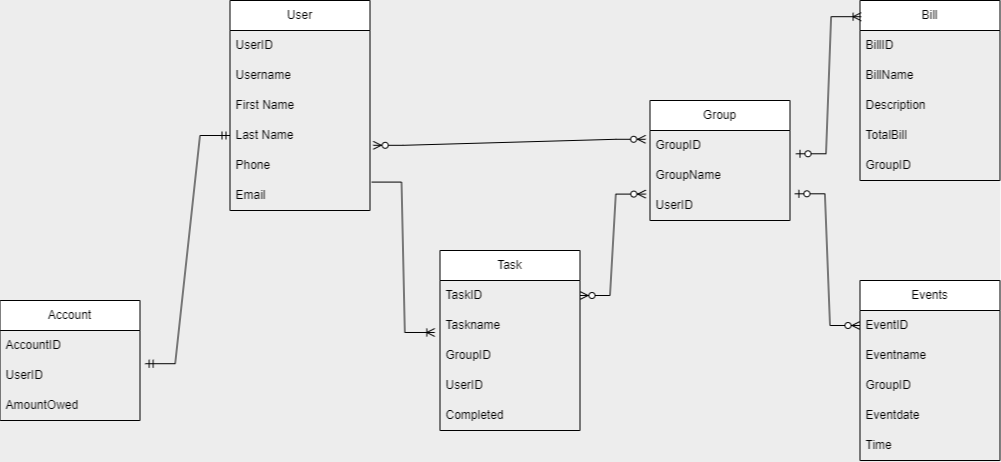
\includegraphics[width=\linewidth]{Database.png}
\caption{Entity-Relationship Diagram of the Housemates Database}
\label{FigDB}
\end{figure}
% Put database relational diagram here

\subsection{Interface Specification} \label{Interface}

In this section, the description of the user interface of \progname{} will be provided. The user interface of \progname{} is designed to be minimalist and simple to use. This will allow the users of \progname{} to quickly access the main functions of \progname{}. Some examples of the interface are described in the figures below and at \url{https://www.figma.com/file/lMZxonql0nhowgpIslIwns/Housemates-Interface-Design?type=design&node-id=0%3A1&mode=design&t=iuU1JQzgxRP93dCL-1}. The interface for \progname{} may change in the final implementation.

\begin{figure}[H]
\centering
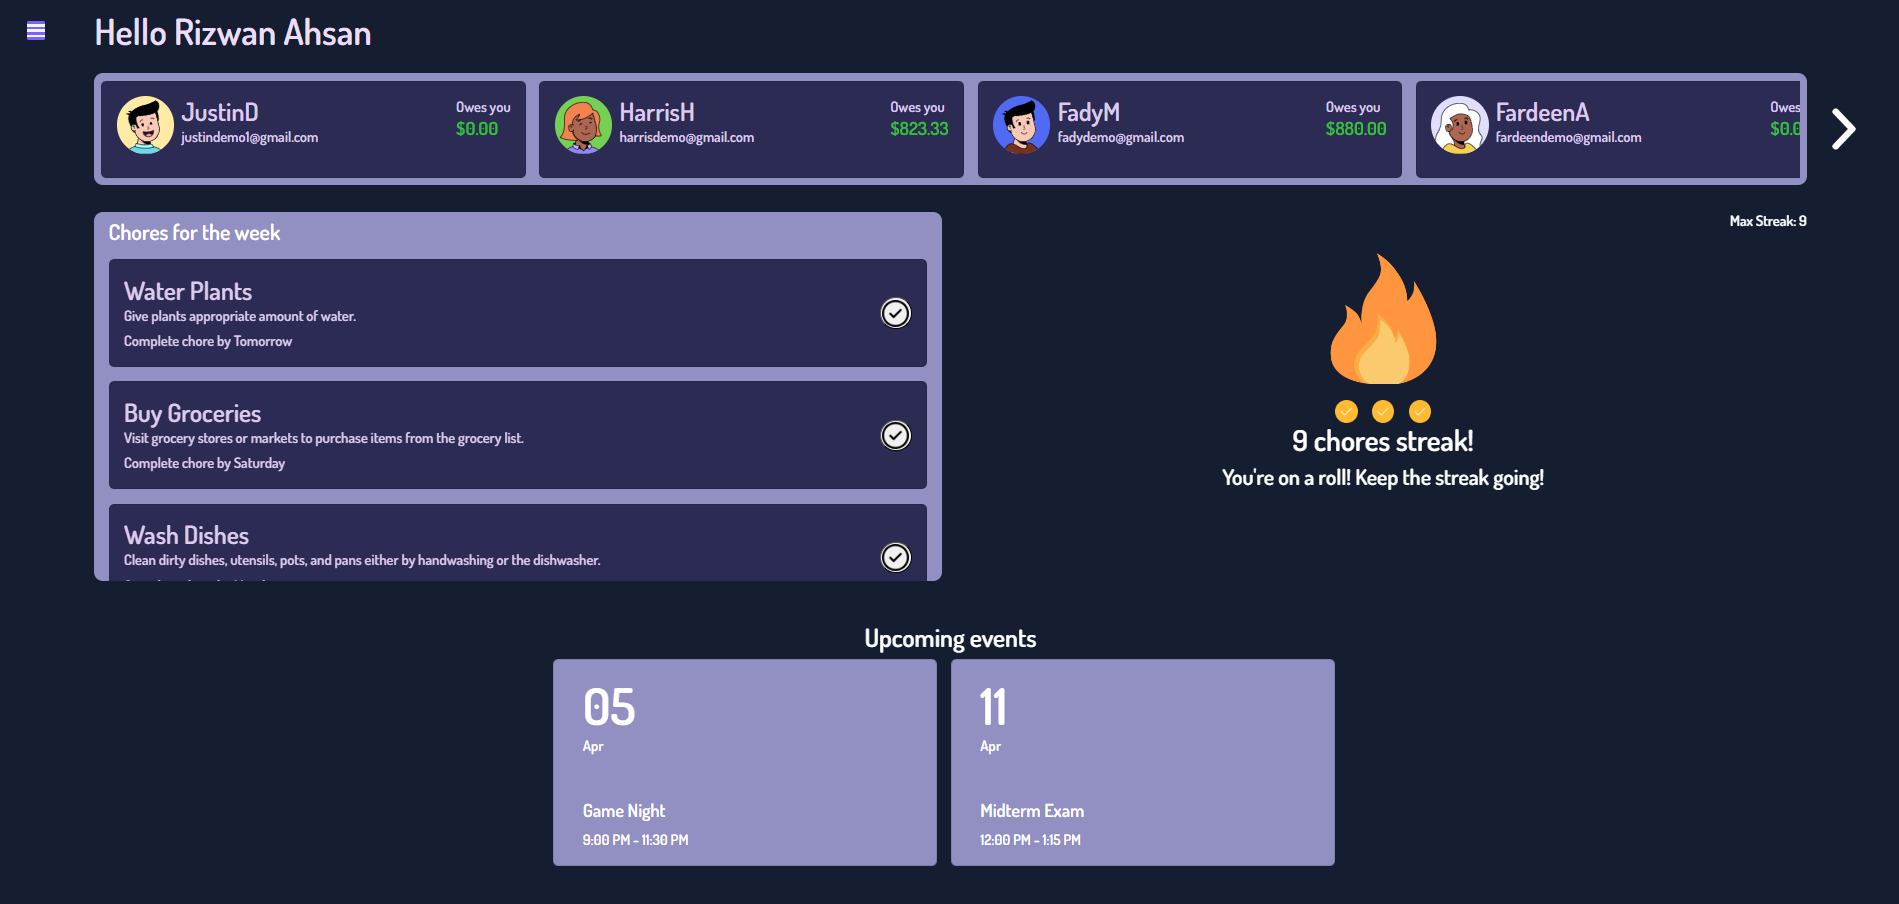
\includegraphics[width=0.25\textwidth]{Homescreen.png}
\caption{Homescreen of \progname{}}
\label{FigHome}
\end{figure}

\begin{figure}[H]
\centering
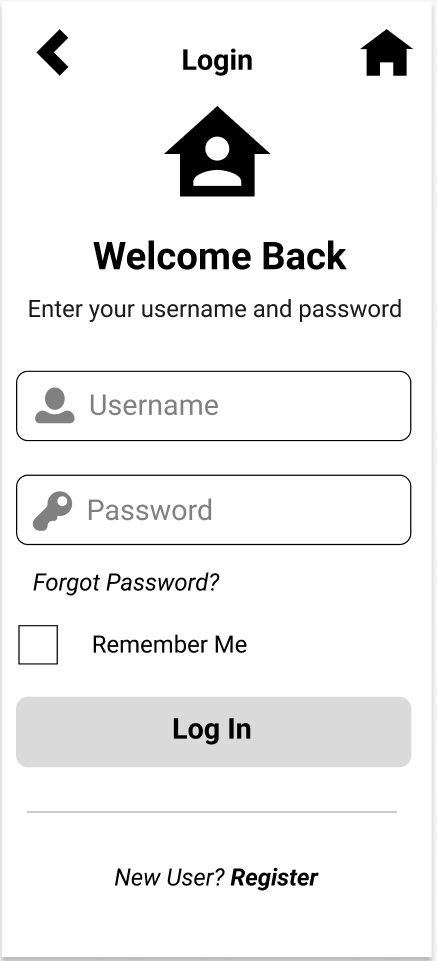
\includegraphics[width=0.25\textwidth]{Login.png}
\caption{Login screen of \progname{}}
\label{FigLogin}
\end{figure}

\begin{figure}[H]
\centering
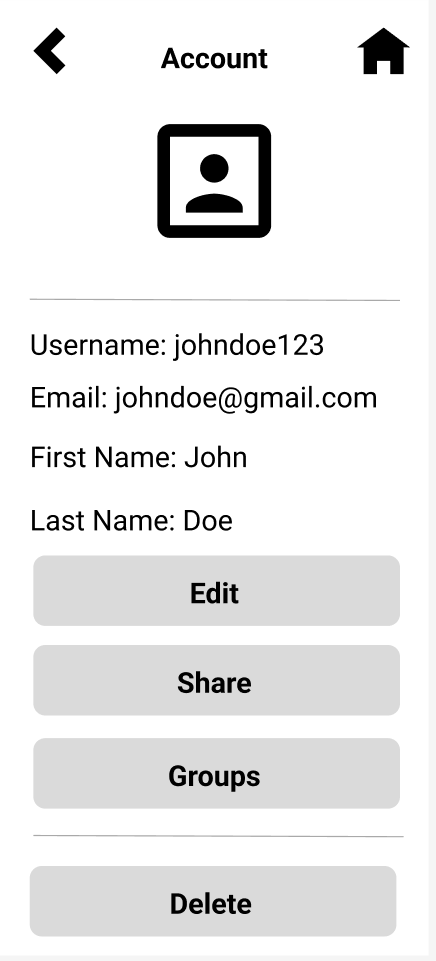
\includegraphics[width=0.25\textwidth]{Account.png}
\caption{Account screen of \progname{}}
\label{FigAccount}
\end{figure}


\begin{figure}[H]
\centering
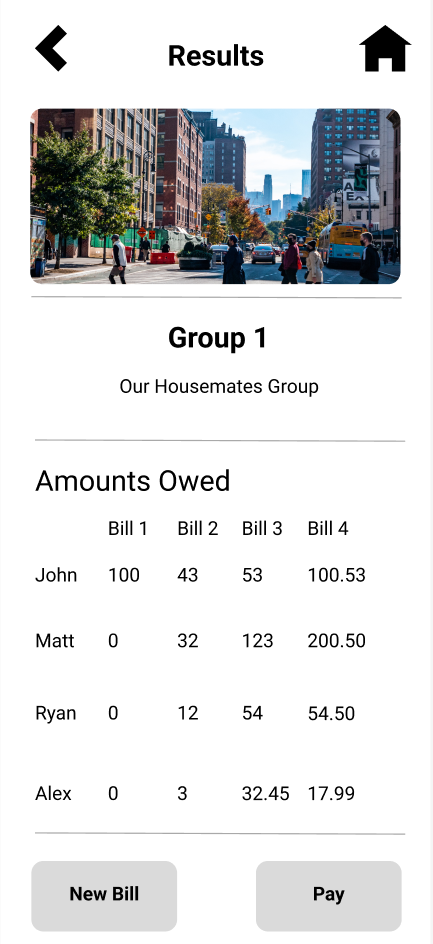
\includegraphics[width=0.25\textwidth]{Bills.png}
\caption{Bills screen of \progname{}}
\label{FigBills}
\end{figure}

\begin{figure}[H]
\centering
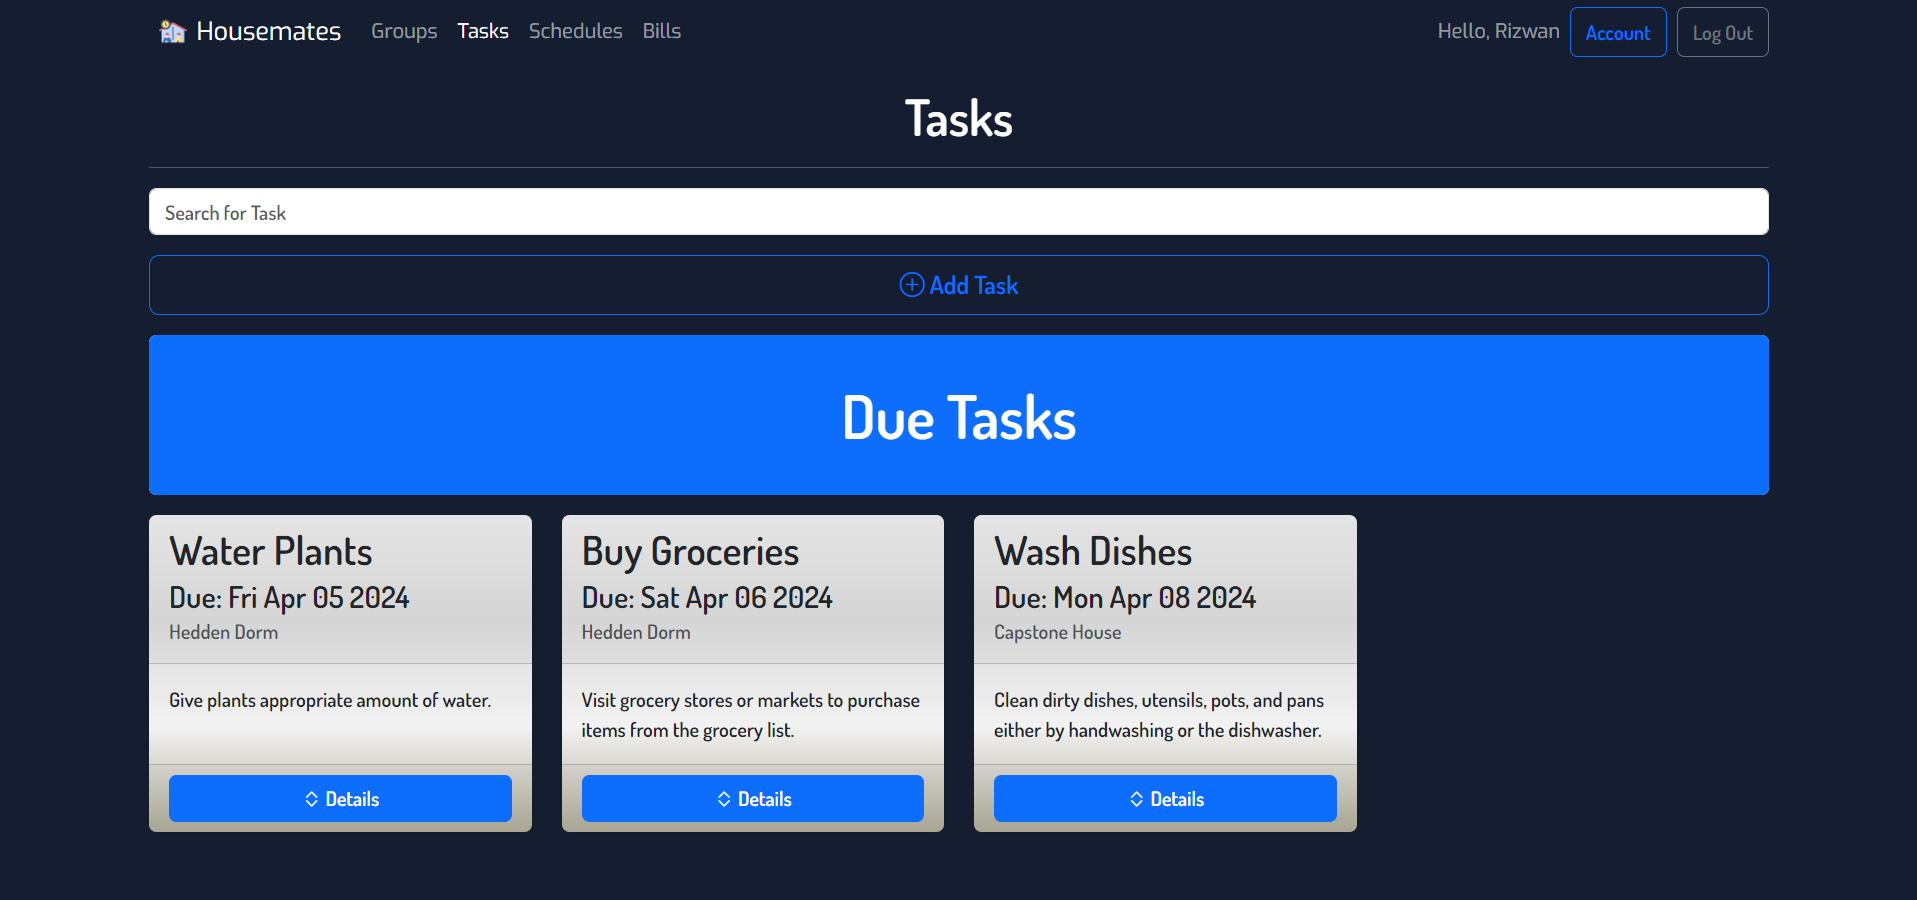
\includegraphics[width=0.25\textwidth]{Task.png}
\caption{Add tasks screen of \progname{}}
\label{FigTasks}
\end{figure}

\begin{figure}[H]
\centering
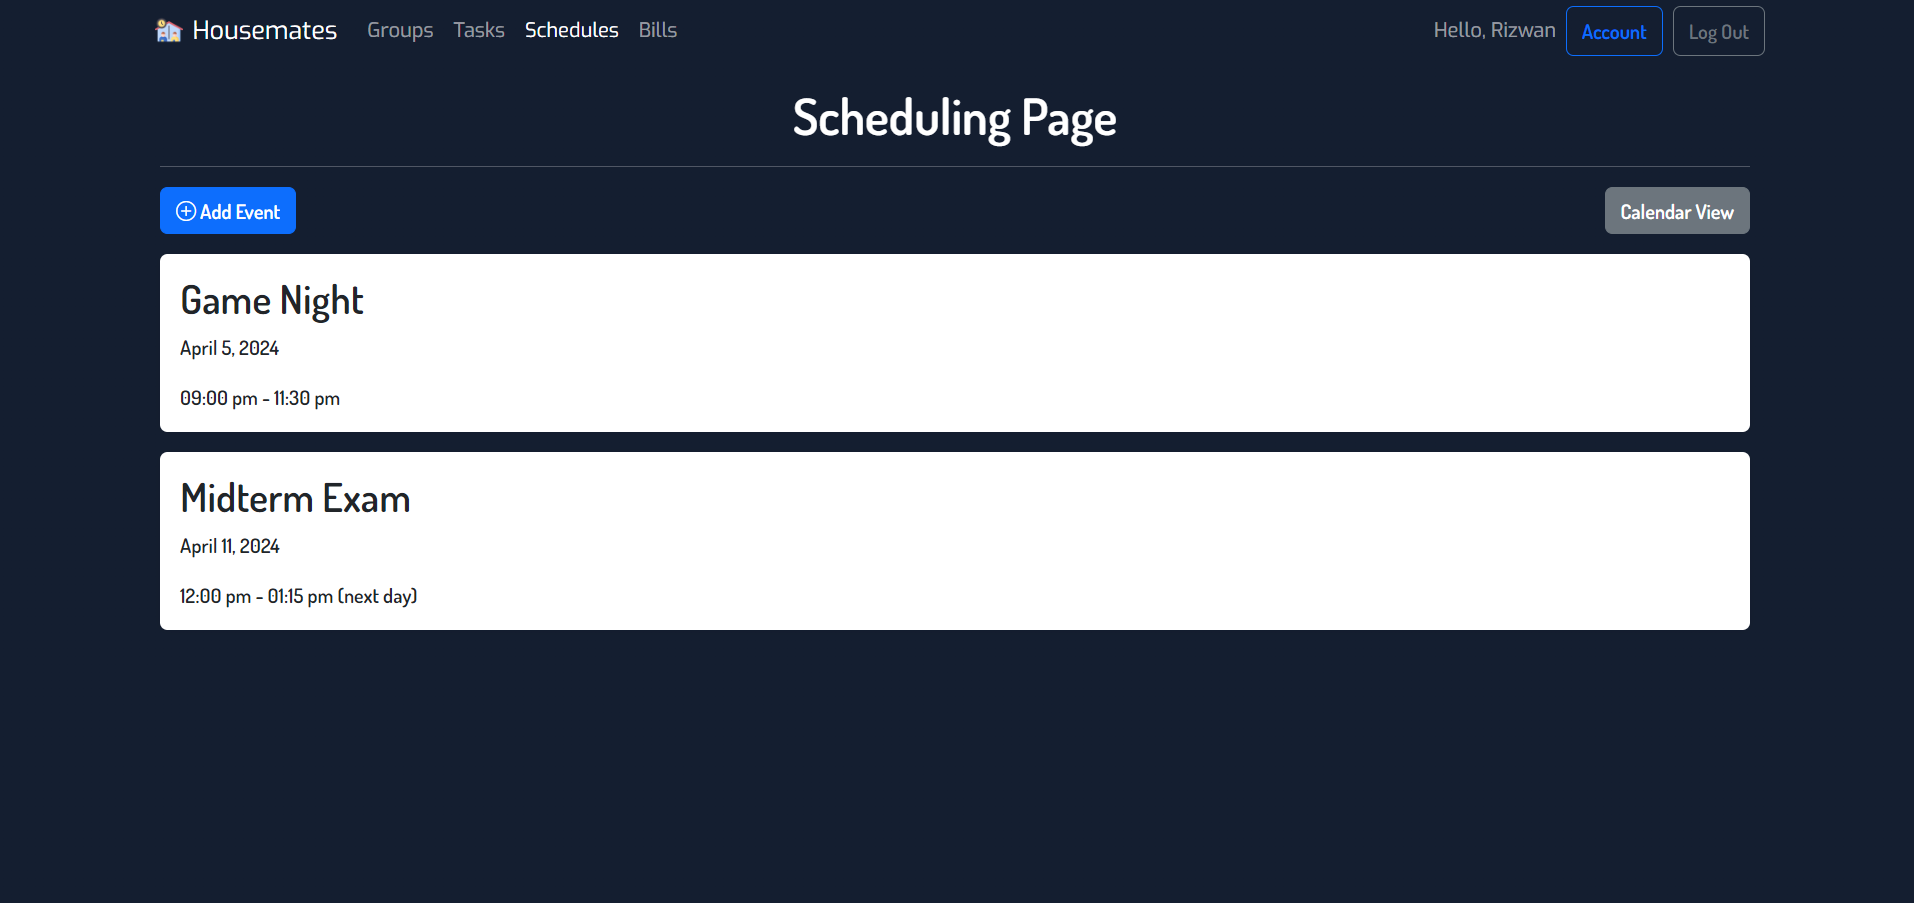
\includegraphics[width=0.25\textwidth]{Events.png}
\caption{Events screen of \progname{}}
\label{FigEvents}
\end{figure}

% \wss{Extra information if required}

\end{document}